
\documentclass[cn]{elegantpaper}

\title{Example of Converting Markdown to \LaTeX{} File \\ Markdown 转为 \LaTeX{} 示例}

\author{邓 东 升}
\date{\today}
\usepackage[nodisplayskipstretch]{setspace}
\usepackage{minted}
\usepackage{mdframed}
\usepackage{xcolor}
\definecolor{fpp2}{RGB}{59, 85, 110}
\definecolor{egray}{RGB}{51, 51, 51}
\definecolor{mgray}{RGB}{243, 243, 243}
\BeforeBeginEnvironment{minted}{\begin{mdframed}[backgroundcolor=mgray,hidealllines=true,innertopmargin=-5pt,innerbottommargin=8pt]}
\AfterEndEnvironment{minted}{\end{mdframed}}
% \setminted{bgcolor=mgray}
% \makeatletter
% \patchcmd{\minted@colorbg}{\noindent}{\medskip\noindent}{}{}
% \apptocmd{\endminted@colorbg}{\par\medskip}{}{}
% \makeatother
\AtBeginEnvironment{minted}{
	\setlength{\parskip}{0pt}
	\singlespacing
	}
\usepackage{ulem}

\begin{document}

\maketitle

\section{Vinaque sanguine metuenti cuiquam Alcyone fixus}

\subsection{This is the section of font shape and face }

Italic font shape is given by \textit{italic text}, and bold face is by \textbf{bold text} or \textbf{bold text},


\textit{Lorem markdownum Letoia}, et alios: figurae \textbf{flectentem} annis aliquid Peneosque ab
esse, obstat gravitate. Obscura atque \textbf{coniuge}, per de coniunx, sibi \textbf{medias
commentaque virgine anima tamen comitemque petis, sed. In Amphion vestros
hamos ire arceor mandere spicula }, in licet aliquando.

\textit{斜体} 中文输入 \textbf{加粗}

\subsection{Highlight of code}

With the language specified (Java), it produce

\begin{minted}{java}
public class Example implements LoremIpsum {
    public static void main(String[] args) {
        if(args.length < 2) {
            System.out.println("Lorem ipsum dolor sit amet");
        }
    } // Obscura atque coniuge, per de coniunx
}
\end{minted}

With the language not specified, it use default highlight scheme for LaTeX. 

\begin{minted}{tex}
\documentclass{elegantpaper}

\author{Dongsheng Deng}
\title{Example of Convert2Read}
\date{\today}

\begin{document}

\maketitle

Hello World.

\end{document}
\end{minted}

For \textbf{inline code highlight}, it's more convenient. for example, \mintinline{tex}{\textbf}.

Te concepit pollice fugit vias alumno \textbf{oras} quam potest \href{http://example.com#rursus}{rursus} optat. Non evadere orbem equorum, spatiis,
vel pede inter si.

\subsection{List }

\textbf{Numbered list} with start 1. 2. and etc.

\begin{enumerate}
  \item De neque iura aquis
  \item Frangitur gaudia mihi eo umor terrae quos
  \item Recens diffudit ille tantum
\end{enumerate}

\textbf{有序列表} 以数字 1. 2. 等开头

\begin{enumerate}
  \item 这是中文列表 1
  \item 这是中文列表 2
  \item 这是中文列表 3
\end{enumerate}

\textbf{无序列表} 以 + 或者 - 开头

\begin{itemize}
  \item 床前明月光
  \item 疑是地上霜
  \item 落霞与孤鹜齐飞
\end{itemize}

\textbf{Un-Numbered list} start with + or -

\begin{itemize}
  \item De neque iura aquis
  \item Frangitur gaudia mihi eo umor terrae quos
  \item Recens diffudit ille tantum
\end{itemize}

\begin{itemize}
  \item De neque iura aquis
  \item Frangitur gaudia mihi eo umor terrae quos
  \item Recens diffudit ille tantum
\end{itemize}

\subsection{Pictures}

You can insert a image using 

\begin{figure}[htbp]
\centering
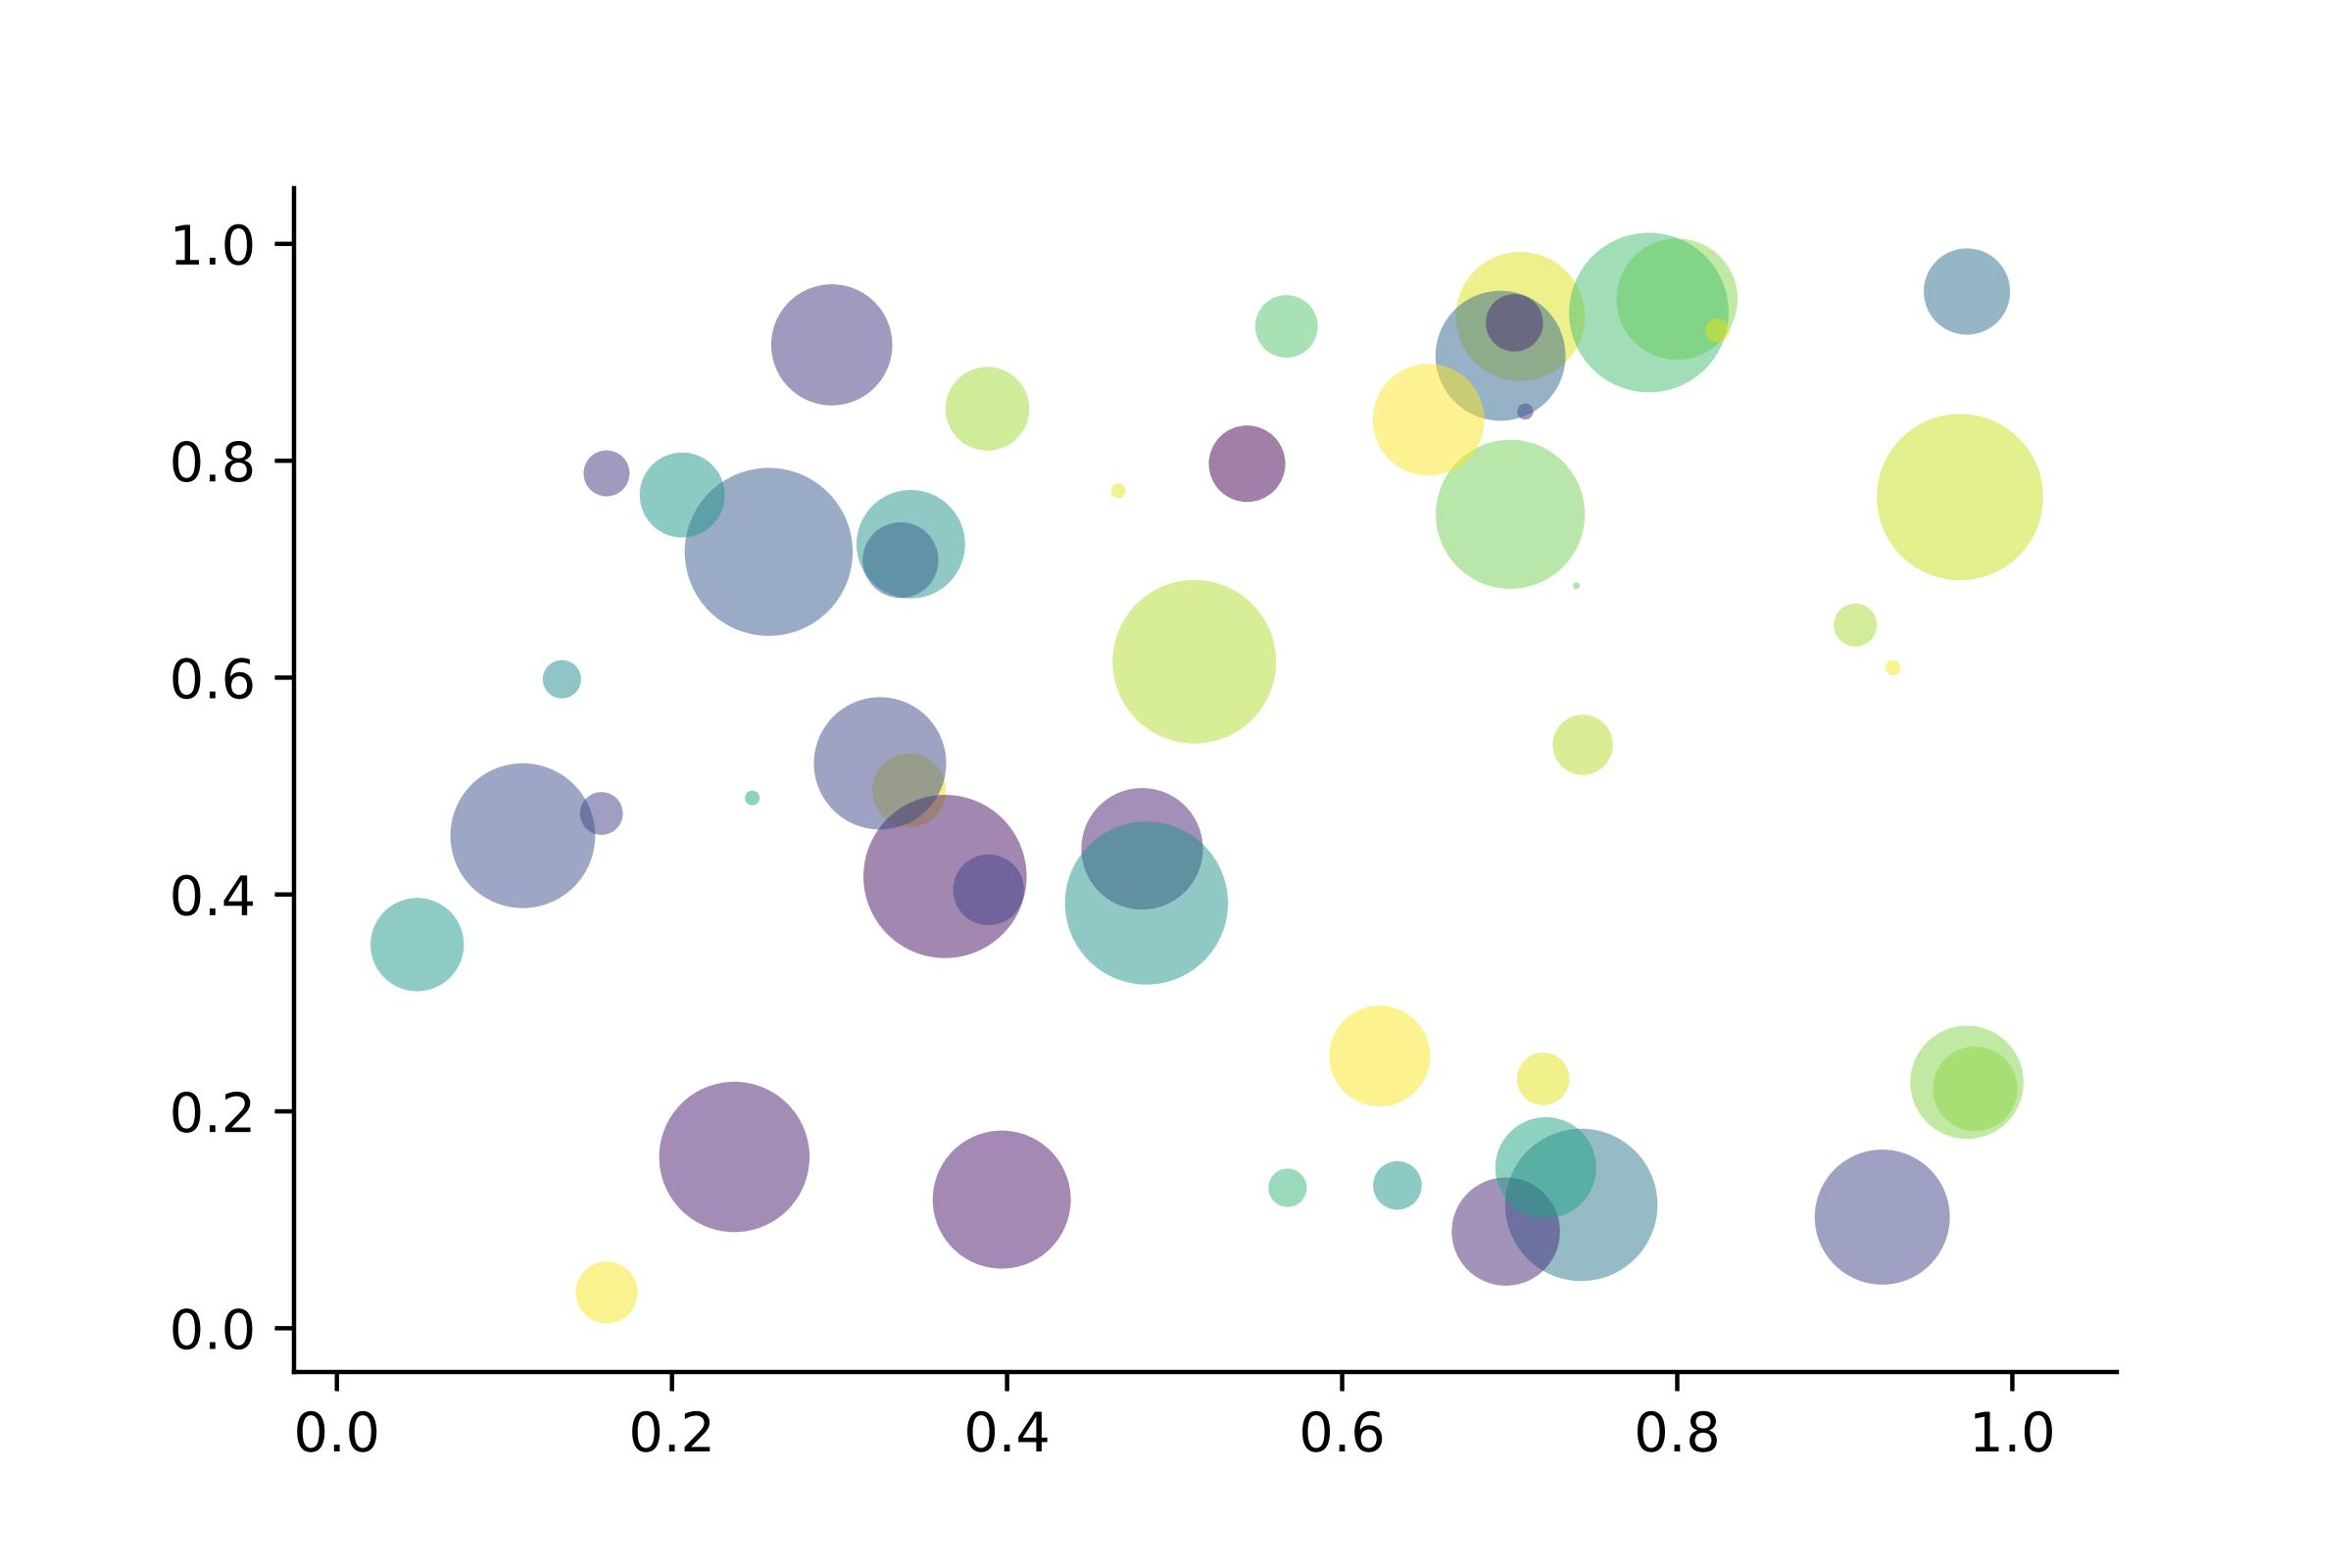
\includegraphics[width=0.7\textwidth]{scatter.jpg}
\caption{Caption}
\end{figure}

The first optional argument is the caption of figure.

\subsection{Equation }

we don't change the content of equation in markdown.

\begin{equation}
a^2 + b^{2} = c_{2} \sum_{i=1}^{T} f(x) \, dx
\end{equation}

\subsection{Links}

The format of link is given by Et nepotes poterat, se qui. Euntem ego pater desuetaque aethera Maeandri, et \href{http://example.com#Dardanio_geminaque}{Dardanio geminaque} cernit. 

\subsection{Quote environment}

Quote environment starts with \mintinline{tex}{>}, 

\begin{quote}
Et nepotes poterat, se qui. Euntem ego pater desuetaque aethera Maeandri. Lassaque poenas nec, manifesta $\pi r^2$ mirantia captivarum prohibebant scelerato gradus unusque dura.
\end{quote}

\begin{quote}
爱因斯坦曾说过 “他没说过这句话”。
\end{quote}





\end{document}
